\chapter{文法与语言}
\section{文法}
\subsection{乔姆斯基体系}
乔姆斯基体系是计算机科学中刻画形式文法表达能力的一个分类谱系,是由诺姆·乔姆斯基于1956年提出的
\cite{DBLP:journals/tit/Chomsky56}。
它包括四个层次:
\begin{itemize}
  \item 0-型文法(无限制文法或短语结构文法)包括所有的文法。该类型的文法能够产生所有可被图灵机识别的语言。
    可被图灵机识别的语言是指能够使图灵机停机的字串,这类语言又被称为递归可枚举语言。
    注意递归可枚举语言与递归语言的区别,后者是前者的一个真子集,是能够被一个总停机的图灵机判定的语言。

  \item 1-型文法(上下文相关文法)生成上下文相关语言。这种文法的产生式规则取如 $ \alpha A \beta \rightarrow \alpha \gamma \beta $
    一样的形式。这里的$A$是非终结符号,而 $\alpha$, $\beta$ 和 $\gamma$ 是包含非终结符号与终结符号的字串;
    $\alpha$, $\beta$ 可以是空串,但 $\gamma$ 必须不能是空串;这种文法也可以包含规则 $S \rightarrow \epsilon$ ,
    但此时文法的任何产生式规则都不能在右侧包含 $S$ 。这种文法规定的语言可以被线性有界非确定图灵机接受。

  \item 2-型文法(上下文无关文法)生成上下文无关语言。这种文法的产生式规则取如 $A \rightarrow \gamma$ 一样的形式。
    这里的$A$是非终结符号,$\gamma$ 是包含非终结符号与终结符号的字串。这种文法规定的语言可以被非确定下推自动机接受。
    上下文无关语言为大多数程序设计语言的语法提供了理论基础。

  \item 3-型文法(正规文法)生成正规语言。这种文法要求产生式的左侧只能包含一个非终结符号,
    产生式的右侧只能是空串、一个终结符号或者一个终结符号后随一个非终结符号;如果所有产生式的右侧都不含初始符号$S$,
    规则 $ S \rightarrow \epsilon$ 也允许出现。这种文法规定的语言可以被有限状态自动机接受,也可以通过正则表达式来获得。
    正规语言通常用来定义检索模式或者程序设计语言中的词法结构。
\end{itemize}

正规语言类包含于上下文无关语言类,上下文无关语言类包含于上下文相关语言类,上下文相关语言类包含于递归可枚举语言类。
如\cref{fig:ChomskyVenn} 所示,这里的包含都是集合的真包含关系,也就是说:存在递归可枚举语言不属于上下文相关语言类,
存在上下文相关语言不属于上下文无关语言类,存在上下文无关语言不属于正规语言类
\cite{DBLP:journals/iandc/Chomsky59a}。

\cref{tab:ChomskyModels} 总结了上述四种类型的文法的主要特点:
\begin{table}[H]
  \centering
  \caption{乔姆斯基体系}
  \label{tab:ChomskyModels}
  \begin{tabular}{|l|l|l|l|}
    \hline
    文法 & 语言 & 自动机 & 产生规则 \\
    \hline
    0-型 & 递归可枚举语言 & 图灵机 & $\alpha \rightarrow \beta$ \\
    \hline
    1-型 & 上下文有关语言 & 线性有界非确定图灵机 & $\alpha A \beta \rightarrow \alpha \gamma \beta$ \\
    \hline
    2-型 & 上下文无关语言 & 非确定下推自动机 & $A \rightarrow \gamma $ \\
    \hline
    3-型 & 正则语言 & 有限状态机 &
    {$\begin{aligned}
        A & \rightarrow aB \\
        A & \rightarrow a
    \end{aligned}$} \tabularnewline
    \hline
  \end{tabular}
\end{table}

\begin{figure}[H]
  \centering
  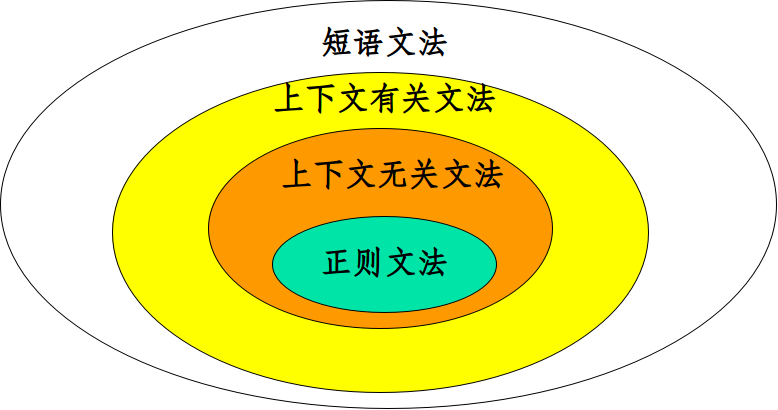
\includegraphics[width=0.68\textwidth]{figure/chomsky_model.png}
  \caption{乔姆斯基体系的韦恩图}
  \label{fig:ChomskyVenn}
\end{figure}

\section{正则文法}
\def\DFA{确定性有限自动机}
正则文法是\emph{\DFA} 识别的文法,是正则表达式的理论基础。\DFA 、正则文法和正则表达式三者是等价的。
\DFA $\mathcal{A}$ 是由:
\begin{itemize}
  \item 一个非空有限状态集合$Q$
  \item 一个输入字母表$\Sigma$(非空有限的字符集合)
  \item 一个转移函数 $ \delta: Q \times \Sigma \rightarrow Q $
    (例如: $ \delta(q, \sigma) = p, (p, q \in Q, \sigma \in \Sigma) $)
  \item 一个开始状态 $ s \in Q $
  \item 一个接受状态 $ F \subset Q $
\end{itemize}
所组成的5-元组。因此一个\DFA 可以写作这样的形式:
$ \mathcal{A} = (Q, \Sigma, \delta, s, F) $。

下面是一个\DFA 的例子。
\begin{figure}[H]
  \centering
  \includesvg[width=0.68\textwidth]{./figure/DFAexample.svg}
  \caption{\DFA 的状态图}
  \label{fig:DFAexample}
\end{figure}
\emph{正则文法} 是产生式规则取下述形式的一种形式文法$ (N, \Sigma, P, S) $:
\begin{enumerate}
  \item $A \rightarrow a$
  \item $A \rightarrow aB$
  \item $C \rightarrow \epsilon$
\end{enumerate}
此处的$A, B, C$是$N$的非终结符号,$a$是$\Sigma$中的终结符号。
这个文法描述的语言也可以用正则表达式$a^{*}bc^{*}$ 来表达。
正规文法描述的语言构成了正规语言类,
正规语言类中的语言也可以由有限状态自动机或正则表达式来表达。

\section{上下文无关文法}
\def\CFGTuple{$G = (N, \Sigma, P, S)$}
\emph{上下文无关文法}(context-free grammar,CFG),
在计算机科学中,若一个形式文法\CFGTuple 的产生式规则都取如下的形式:$V \rightarrow \omega$,其中$ V \in N, \omega \in (N \cup \Sigma)^{*} $,
则称为上下文无关文法。
上下文无关文法取名为“上下文无关”的原因就是因为字符 $V$ 总可以被字串 $\omega$ 自由替换,而无需考虑字符 $V$ 出现的上下文。
一个形式语言是上下文无关的,如果它是由上下文无关文法生成的。

上下文无关文法重要的原因在于它们拥有足够强的表达力来表示大多数程序设计语言的语法;
实际上,几乎所有程序设计语言都是通过上下文无关文法来定义的。
另一方面,上下文无关文法又足够简单,
使得我们可以构造有效的分析算法来检验一个给定字串是否是由某个上下文无关文法产生的,如LL分析器和LR分析器。

BNF(巴克斯-诺尔范式)经常用来表达上下文无关文法。

上下文无关文法$G$是4-元组:
\begin{equation*}
  G = (V, \Sigma, R, S)
\end{equation*}
\begin{enumerate}
  \item $V$ 是``非终结''符号或变量的有限集合。它们表示在句子中不同类型的
    短语或句子。
  \item $\Sigma$ 是``终结符''的有限集合,与$V$没有交集,它们构成了句子的
    实际内容。
  \item $S$是开始变量,用来表示整个句子(或程序)。它必须是$V$的元素。
  \item $R$是从$V$到$(V\cup\Sigma)^{*}$ 的关系,使得
    $ \exists \omega \in (V\cup\Sigma)^{*}: (S,\omega) \in R$。
\end{enumerate}
此外,$R$是有限集合。$R$的成员叫做文法的``规则''或者``产生式''。星号表示
\emph{Kleene星号}运算符。
例子:
\begin{lstlisting}
S ::= T '+' S | T '-' S | T
T ::= T '*' T | T '/' T | '(' S ')' | x | y | z
\end{lstlisting}
例如字符串\texttt{(x + y) * x - z * y / (x + x)}就可以用这个文法产生。
